\whiteBGstarBegin
\setcounter{section}{0}
\begin{enumerate}[label=\bfseries Câu \arabic*:]
	
	\item \mkstar{1} [4]
	
	\cauhoi{
		Hệ thức nào sau đây phù hợp với định luật Sác-lơ?
		\begin{mcq}(4)
			\item $p\sim t$.
			\item $\dfrac{p_1}{T_1} = \dfrac{p_2}{T_2}$.
			\item $\dfrac{p}{t} = \text{hằng số}$.
			\item $\dfrac{p_1}{p_2} = \dfrac{T_2}{T_1}$.
		\end{mcq}
	}
	
	\loigiai{
		\textbf{Đáp án: B.}
		
		Hệ thức phù hợp với định luật Sác-lơ là $\dfrac{p}{T} = \text{hằng số}$, hoặc $\dfrac{p_1}{T_1} = \dfrac{p_2}{T_2}$, với $T$ viết in hoa chỉ nhiệt độ tuyệt đối.
	}
	
	\item \mkstar{1} [5]
	
	\cauhoi{
		Quá trình biến đổi trạng thái trong đó thể tích được giữ không đổi gọi là quá trình
		\begin{mcq}(4)
			\item đẳng nhiệt. 
			\item đẳng áp.
			\item đoạn nhiệt.
			\item đẳng tích.
		\end{mcq}
		
	}
	
	\loigiai{
		\textbf{Đáp án: D.}
		
		Quá trình biến đổi trạng thái trong đó thể tích được giữ không đổi gọi là quá trình đẳng tích.
	}

		\item \mkstar{1} [5]

\cauhoi{
	Trong các hệ thức sau, hệ thức nào \textbf{không} phù hợp với quá trình đẳng tích?
	\begin{mcq}(4)
		\item $p\sim t$. 
		\item $p\sim T$.
		\item $\dfrac{p_1}{T_1} = \dfrac{p_2}{T_2}$.
		\item $\dfrac{p}{T} = \text{hằng số}$.
	\end{mcq}
	
}

\loigiai{
	\textbf{Đáp án: A.}
	
	Hệ thức phù hợp với định luật Sác-lơ là $\dfrac{p}{T} = \text{hằng số}$, hoặc $\dfrac{p_1}{T_1} = \dfrac{p_2}{T_2}$, với $T$ viết in hoa chỉ nhiệt độ tuyệt đối.
	
	Vậy $p\sim t$ không phù hợp với quá trình đẳng tích.
}
		\item \mkstar{1} [24]

\cauhoi{
	Quá trình đẳng tích là quá trình biến đổi trạng thái trong đó
	\begin{mcq}(2)
		\item nhiệt độ được giữ không đổi. 
		\item áp suất được giữ không đổi.
		\item lực nén được giữ không đổi.
		\item thể tích được giữ không đổi.
	\end{mcq}
	
}

\loigiai{
	\textbf{Đáp án: D.}
	
	Quá trình đẳng tích là quá trình biến đổi trạng thái trong đó thể tích được giữ không đổi.
}
		\item \mkstar{1} [32]

\cauhoi{
	Trong hệ tọa độ ($p,T$) đường biểu diễn nào sau đây là đường đẳng tích?
	\begin{mcq}
		\item Đường hyperbol.
		\item Đường thẳng kéo dài đi qua gốc tọa độ.
		\item Đường thẳng kéo dài không đi qua gốc tọa độ.
		\item Đường thẳng cắt trục $p$ tại điểm $p=p_0$.
	\end{mcq}
	
}

\loigiai{
	\textbf{Đáp án: B.}
	
	Trong hệ tọa độ ($p,T$) đường đẳng tích là đường thẳng kéo dài đi qua gốc tọa độ.
}
		\item \mkstar{2} [5]
	
	\cauhoi{
		Một khối khí lí tưởng đang ở nhiệt độ $\SI{37}{\celsius}$, áp suất $\SI{4}{atm}$ thì được làm lạnh đẳng tích cho đến khi áp suất còn $\SI{2}{atm}$. Nhiệt độ của khối khí lúc đó bằng
		\begin{mcq}(4)
			\item $\SI{-118}{\celsius}$. 
			\item $\SI{775}{\celsius}$.
			\item $\SI{155}{\celsius}$.
			\item $\SI{129}{\celsius}$.
		\end{mcq}
		
	}
	
	\loigiai{
		\textbf{Đáp án: A.}
		
		Đẳng tích (1): $p_1=\SI{4}{atm}$, $T_1=\SI{310}{K}$ sang (2): $p_2=\SI{2}{atm}$, $T_2=?$
		
		Vì quá trình là đẳng tích nên ta có phương trình:
		
		$$\dfrac{p_1}{T_1} = \dfrac{p_2}{T_2} \Rightarrow T_2 =\dfrac{T_1p_2}{p_1} = \SI{155}{K}.$$
		
		Đổi $t_2 = T_2 - 273 = \SI{-118}{\celsius}$.
	}



		\item \mkstar{2} [5]
	
	\cauhoi{
		Một lốp ô tô chứa không khí ở áp suất $\SI{5}{bar}$, nhiệt độ $\SI{25}{\celsius}$. Khi xe chạy, nhiệt độ trong lốp tăng lên đến $\SI{50}{\celsius}$, áp suất không khí trong lốp khi đó là
		\begin{mcq}(4)
			\item $\SI{10.45}{bar}$. 
			\item $\SI{10}{bar}$.
			\item $\SI{5.42}{bar}$.
			\item $\SI{4.55}{bar}$.
		\end{mcq}
		
	}
	
	\loigiai{
		\textbf{Đáp án: C.}
		
			Đẳng tích (1): $p_1=\SI{5}{bar}$, $T_1=\SI{298}{K}$ sang (2): $p_2=?$, $T_2=\SI{323}{K}$
		
		Vì quá trình là đẳng tích nên ta có phương trình:
		
		$$\dfrac{p_1}{T_1} = \dfrac{p_2}{T_2} \Rightarrow p_2 =\dfrac{p_1T_2}{T_1} = \SI{5.42}{bar}.$$
	}



		\item \mkstar{2} [24]
	
	\cauhoi{
		Quá trình nào sau đây có thể xem là quá trình đẳng tích?
		\begin{mcq}
			\item Thổi không khí vào một quả bóng bay. 
			\item Đun nóng khí trong một xi lanh có pit-tông cố định.
			\item Đun nóng khí trong một xi lanh có pit-tông không cố định.
			\item Quả bóng bàn bị bẹp nhúng vào nước nóng, phồng lên như cũ.
		\end{mcq}
		
	}
	
	\loigiai{
		\textbf{Đáp án: B.}
		
		Đun nóng khí trong một xi lanh có pit-tông cố định thì thể tích khí bên trong không đổi, do đó có thể xem là quá trình đẳng tích.
	}

		\item \mkstar{2} [24]
	
	\cauhoi{
		Một khối khí lí tưởng được đựng trong bình kín. Sau khi khối khí được đun nóng, nhiệt độ tuyệt đối của khối khí là $\SI{360}{K}$ và áp suất của khối khí tăng gấp 1,2 lần. Nhiệt độ tuyệt đối ban đầu của khối khí là
		\begin{mcq}(4)
			\item $\SI{60}{K}$. 
			\item $\SI{72}{K}$.
			\item $\SI{300}{K}$.
			\item $\SI{360}{K}$.
		\end{mcq}
		
	}
	
	\loigiai{
		\textbf{Đáp án: C.}
		
		Đẳng tích (1): $p_1$, $T_1=?$ sang (2): $p_2=1,2p_1$, $T_2=\SI{360}{K}$
		
		Vì quá trình là đẳng tích nên ta có phương trình:
		
		$$\dfrac{p_1}{T_1} = \dfrac{p_2}{T_2} \Rightarrow T_1 =\dfrac{p_1T_2}{p_2} = \SI{300}{bar}.$$
	}

		\item \mkstar{2} [29]
	
	\cauhoi{
		Ở điều kiện tiêu chuẩn, chất khí ở $\SI{0}{C}$ có áp suất $\SI{1}{atm}$. Coi thể tích của chất khí là không đổi, áp suất khí ở $\SI{47}{\celsius}$ có giá trị xấp xỉ bằng
		\begin{mcq}(4)
			\item $\SI{1.17}{atm}$. 
			\item $\SI{1.56}{atm}$.
			\item $\SI{1.92}{atm}$.
			\item $\SI{1.25}{atm}$.
		\end{mcq}
		
	}
	
	\loigiai{
		\textbf{Đáp án: A.}
		
		Đẳng tích (1): $p_1=\SI{1}{atm}$, $T_1=\SI{273}{K}$ sang (2): $p_2=?$, $T_2=\SI{320}{K}$
		
		Vì quá trình là đẳng tích nên ta có phương trình:
		
		$$\dfrac{p_1}{T_1} = \dfrac{p_2}{T_2} \Rightarrow p_2 =\dfrac{p_1T_2}{T_1} = \SI{1.17}{atm}.$$
	}


	
	\item \mkstar{1} [2]
	
	\cauhoi{
		Quá trình đẳng tích là gì? Phát biểu và viết công thức định luật liên quan. Vẽ đường đẳng tích trong hệ trục ($p,T$) với $\text{O}T$ là trục hoành.
	}
	
	\loigiai{		
		Quá trình biến đổi trạng thái mà trong đó thể tích được giữ không đổi gọi là quá trình đẳng tích.
		
		Trong quá trình đẳng tích, áp suất tỉ lệ thuận với nhiệt độ tuyệt đối.
		
		Công thức định luật Sác-lơ: $p\sim T$ hay $\dfrac{p}{T} = \text{hằng số}$ hay $\dfrac{p_1}{T_1}=\dfrac{p_2}{T_2}$.
		
		Đường đẳng tích trong hệ trục ($p,T$) với $\text{O}T$ là trục hoành:
		\begin{center}
			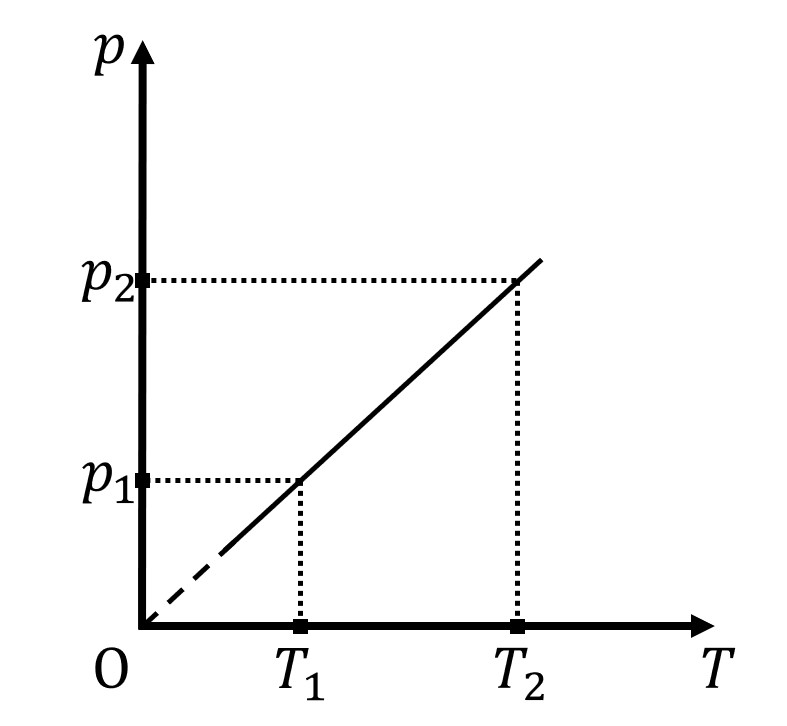
\includegraphics[scale=0.4]{../figs/VN10-PH-39-L-0293-4.jpg}
		\end{center}
	}
	
	
	\item \mkstar{2} [3]
	
	\cauhoi{
		Xét lượng khí xác định chứa trong bình kín có thể tích $V$ không đổi. Khi tăng nhiệt độ tuyệt đối thì áp suất của lượng khí thay đổi như thế nào (tăng hay giảm)? Giải thích.
	}
	
	\loigiai{
		Trong quá trình đẳng tích, áp suất tỉ lệ thuận với nhiệt độ tuyệt đối. Vậy khi tăng nhiệt độ tuyệt đối thì áp suất của lượng khí tăng.
	}
	
	\item \mkstar{2} [7]
	
	\cauhoi{
		Một lượng khí hidro đựng trong bình kín có thể tích không đổi. Ở áp suất $\SI{1.5}{atm}$ thì nhiệt độ của khối khí là $\SI{27}{\celsius}$.
		\begin{enumerate}[label=\alph*)]
			\item Tính áp suất của khí khi đun nóng đến $\SI{127}{\celsius}$.
			\item Để áp suất của khí là $\SI{3}{atm}$ thì phải đun nóng đến bao nhiêu độ C?
		\end{enumerate}
	}
	
	\loigiai{
		\begin{enumerate}[label=\alph*)]
			\item Tính áp suất của khí khi đun nóng đến $\SI{127}{\celsius}$.
			
			Đẳng tích (1): $p_1=\SI{1.5}{atm}$, $T_1=\SI{300}{K}$ sang (2): $p_2=?$, $T_2=\SI{400}{K}$
			
			Vì quá trình là đẳng tích nên ta có phương trình:
			
			$$\dfrac{p_1}{T_1} = \dfrac{p_2}{T_2} \Rightarrow p_2 =\dfrac{p_1T_2}{T_1} = \SI{2}{atm}.$$
			
			\item Để áp suất của khí là $\SI{3}{atm}$ thì phải đun nóng đến bao nhiêu độ C?.
			
			Đẳng tích (1): $p_1=\SI{1.5}{atm}$, $T_1=\SI{300}{K}$ sang (2): $p_2=\SI{3}{atm}$, $T_2=?$
			
			Vì quá trình là đẳng tích nên ta có phương trình:
			
			$$\dfrac{p_1}{T_1} = \dfrac{p_2}{T_2} \Rightarrow T_2 =\dfrac{p_2T_1}{p_1} = \SI{600}{K}.$$
			
			Đổi $t_2=T_2-273 = \SI{327}{\celsius}$.
		\end{enumerate}
		
	}

	\item \mkstar{2} [8]
	
	\cauhoi{
		Tại sao lốp xe ô tô thường nổ khi xe đang chạy ngoài trời nóng hơn là để xe nằm yên trong gara? Định luật vật lý nào mà em đã học có thể giải thích hiện tượng trên?
	}
	
	\loigiai{
		Khi lốp xe đang chạy trên đường, do ma sát với đường và nắng nóng làm cho nhiệt độ của không khí bên trong lốp xe tăng lên, làm cho áp suất khí trong lốp xe tăng lên theo (quá trình đẳng tích). Khi áp suất tăng đến một mức nào đó thì có thể gây nổ lốp xe.
		
		Khi để xe trong gara, do nhiệt độ không cao như trường hợp trên nên áp suất khối khí cũng không cao, lốp xe khó nổ hơn.
		
		Giải thích hiện tượng trên, ta dùng định định luật Sác-lơ về quá trình đẳng tích.
		
	}
	\item \mkstar{2} [11]

\cauhoi{
	
	Đun nóng đẳng tích lượng khí lí tưởng từ nhiệt độ tuyệt đối $\SI{150}{K}$, áp suất $\SI{4}{atm}$. Tìm nhiệt độ tuyệt đối của khối khí khi áp suất là $\SI{6}{atm}$.
}

\loigiai{
	Đẳng tích (1): $p_1=\SI{4}{atm}$, $T_1=\SI{150}{K}$ sang (2): $p_2=\SI{6}{atm}$, $T_2=?$
	
	Vì quá trình là đẳng tích nên ta có phương trình:
	
	$$\dfrac{p_1}{T_1} = \dfrac{p_2}{T_2} \Rightarrow T_2 =\dfrac{p_2T_1}{p_1} = \SI{225}{K}.$$
	
}

\item \mkstar{2} [12]

\cauhoi{
	
	Các quả bóng bay là món đồ chơi được trẻ em thích nhưng khí được bơm vào bóng bay thường là hydro, metan hoặc khí đất đèn rất nguy hiểm khi cháy nổ. Hãy giải thích tại sao bóng bay để ngoài trời nắng nóng lại phát nổ?
}

\loigiai{
	
	Khi để ngoài trời nắng nóng thì nhiệt độ tăng, làm cho áp suất khí bên trong quả bóng tăng. Khi áp suất tăng vượt quá giới hạn mà vỏ quả bóng chịu được thì quả bóng phát nổ. Hiện tượng này được giải thích bằng định luật Sác-lơ cho quá trình đẳng tích.
	
}

\item \mkstar{2} [18]

\cauhoi{
	
	Một bóng đèn dây tóc chứa khí trơ, khi đèn sáng nhiệt độ của bóng đèn là $\SI{450}{\celsius}$, áp suất khí trong bóng đèn bằng áp suất khí quyển là $\SI{1}{atm}$. Tính áp suất khí trong bóng đèn khi đèn chưa sáng ở $\SI{22}{\celsius}$.
}

\loigiai{
	Đẳng tích (1): $p_1=\SI{1}{atm}$, $T_1=\SI{723}{K}$ sang (2): $p_2=?$, $T_2=\SI{295}{K}$
	
	Vì quá trình là đẳng tích nên ta có phương trình:
	
	$$\dfrac{p_1}{T_1} = \dfrac{p_2}{T_2} \Rightarrow p_2 =\dfrac{p_1T_2}{T_1} = \SI{1.17}{atm}.$$
	
}

\item \mkstar{2} [22]

\cauhoi{
	
	Vì sao nồi áp suất có thể nấu chín thịt trong một thời gian ngắn?
}

\loigiai{
	Do nồi áp suất có kết cấu kín (thể tích khí bên trong không đổi), khi ở $\SI{100}{\celsius}$, các phân tử hơi nước không thoát được ra ngoài, khí này sẽ bị giữ lại trong nồi ngày càng nhiều, làm cho áp suất không khí trong nồi tăng cao. Khi áp suất tăng dẫn đến điểm sôi (nhiệt độ mà tại đó có sự sôi xảy ra) cũng tăng, nước không thể bị hóa hơi mà buộc phải hấp thụ nhiệt lượng tiếp tục tăng nhiệt độ, luôn giữ ở trạng thái sôi. Trong quá trình này nhiệt lượng được thức ăn hấp thu ngày càng nhiều. Nhiệt độ trong nồi áp suất có thể đạt tới $\SI{120}{\celsius}$, ở nhiệt độ này, thức ăn rất mau chín.
	
}
\item \mkstar{2} [30]

\cauhoi{
	
	\begin{enumerate}[label=\alph*)]
		\item Đẳng quá trình là quá trình biến đổi trạng thái mà trong đó có một thông số không thay đổi. Dựa vào đó, em hãy cho biết thế nào là quá trình đẳng tích?
		\item Trong quá trình đẳng tích, áp suất và nhiệt độ tuyệt đối có mối quan hệ như thế nào?
		\item Một săm xe máy được bơm căng không khí ở nhiệt độ $\SI{20}{\celsius}$ và áp suất $\SI{2}{atm}$. Tính áp suất trong săm xe khi nhiệt độ lên đến $\SI{42}{\celsius}$. Từ đó cho biết săm có bị nổ không nếu coi như sự tăng thể tích của săm là không đáng kể và săm chịu được áp suất tối đa là $\SI{2.5}{atm}$.
	\end{enumerate}
}

\loigiai{
	\begin{enumerate}[label=\alph*)]
		\item Quá trình đẳng tích là quá trình biến đổi trạng thái mà trong đó thể tích không thay đổi.
		\item Trong quá trình đẳng tích, áp suất tỉ lệ thuận với nhiệt độ tuyệt đối.
		\item Đẳng tích (1): $p_1=\SI{2}{atm}$, $T_1=\SI{293}{K}$ sang (2): $p_2=?$, $T_2=\SI{315}{K}$
		
		Vì quá trình là đẳng tích nên ta có phương trình:
		
		$$\dfrac{p_1}{T_1} = \dfrac{p_2}{T_2} \Rightarrow p_2=\dfrac{p_1T_2}{T_1} = \SI{2.15}{atm}.$$
		
		Vì $\SI{2.15}{atm} < \SI{2.5}{atm}$ nên săm không bị nổ.
	\end{enumerate}
	
}
	\item \mkstar{3} [10]
	
	\cauhoi{
		
		Đun nóng đẳng tích một khối khí lên thêm $\SI{10}{\celsius}$ thì áp suất tăng thêm $1/50$ áp suất khí ban đầu. Tìm nhiệt độ ban đầu của khí.
	}
	
	\loigiai{
		Đẳng tích (1): $p_1$, $T_1$ sang (2): $p_2=(1+1/50)p_1$, $T_2=T_1+10$
		
		Vì quá trình là đẳng tích nên ta có phương trình:
		
		$$\dfrac{p_1}{T_1} = \dfrac{p_2}{T_2} \Rightarrow T_1 =\dfrac{p_1T_2}{p_2} = \SI{500}{K}.$$
		
		Đổi $t_1=T_1 - 273 = \SI{227}{\celsius}$.
		
	}



	\item \mkstar{3} [27]
	
	\cauhoi{
		PSI là chỉ số áp suất của không khí bị nén trong lốp xe, được đo bằng đơn vị Pounds trên một Inch vuông (Pounds per Square Inch). PSI thường được ghi trên thành lốp xe, nó cho biết áp suất tối đa mà lốp xe chịu được. Khi bơm hoặc khi kiểm tra lốp, chúng ta phải làm sao cho lớp đủ hơi, tức là có đủ số PSI cần thiết, thiếu quá hoặc thừa quá đều có thể đưa đến tình trạng hại xe, hư lốp, hao mòn và nguy hiểm nhất là nổ lốp, gây ra tai nạn trầm trọng.
			
			Một chiếc lốp sau của xe Vinfast chứa không khí ở áp suất $\SI{40}{PSI}$ (đổi đơn vị $\SI{1}{PSI} \approx \SI{6895}{Pa}$) và nhiệt độ $\SI{27}{\celsius}$. Khi xe chạy nhanh, lốp xe nóng lên làm nhiệt độ không khí trong lốp xe tăng tới $\SI{57}{\celsius}$. Chỉ số PSI an toàn ghi trên lốp xe của dòng xe này là $\SI{46}{PSI}$. Bỏ qua sự dãn nở của lốp xe, hỏi lốp xe có bị nổ không? Vì sao?
		
	
	}
	
	\loigiai{
	
		Đẳng tích (1): $p_1=\SI{40}{PSI}$, $T_1=\SI{300}{K}$ sang (2): $p_2=?$, $T_2=\SI{330}{K}$
		
		Vì quá trình là đẳng tích nên ta có phương trình:
		
		$$\dfrac{p_1}{T_1} = \dfrac{p_2}{T_2} \Rightarrow p_2 =\dfrac{p_1T_2}{T_1} = \SI{44}{PSI}.$$
		
		Vì $\SI{44}{PSI} < \SI{46}{PSI}$ nên lốp xe không bị nổ.
		
	}

	\item \mkstar{3} [28]
	
	\cauhoi{
		Để giảm thiểu thời gian đi lại, vận chuyển sản phẩm giao thương giữa các vùng miền tổ quốc, Việt Nam đã có chủ trương tiến hành xây dựng tuyến đường cao tốc Bắc - Nam với tốc độ tối đa rất cao từ $\SI{80}{km/h} \rightarrow \SI{120}{km/h}$. Đường cao tốc của Việt Nam được xây dựng theo đúng tiêu chuẩn quốc tế, do đó mặt đường sẽ có độ nhám rất cao. Độ bám và ma sát của bánh xe với mặt đường tăng lên giúp hạn chế nguy cơ xảy ra tai nạn nhưng lại khiến lốp xe nhanh bị mài mòn hơn.
		\begin{enumerate}[label=\alph*)]
			\item Nếu em là tài xế chạy trên đường cao tốc, em hãy giải thích tại sao ô tô thường nổ lốp trên đường cao tốc và gây ra rất nhiều tai nạn thương tâm? Nêu biện pháp khắc phục để giảm thiểu tình trạng trên.
			\item Giả sử có một lốp ô tô chịu được áp suất tối đa $\SI{40}{kPa}$. Lốp được bơm đầy không khí ở nhiệt độ $\SI{27}{\celsius}$ với áp suất $\SI{36}{kPa}$. Khi chạy trên đường cao tốc, lốp xe nóng lên tới $\SI{67}{\celsius}$ thì có bị nổ không? Vì sao? (Bỏ qua sự nở vì nhiệt của lốp xe).
		\end{enumerate}
	}
	
	\loigiai{
		\begin{enumerate}[label=\alph*)]
			\item Khi di chuyển trên đường cao tốc, xe chạy với tốc độ càng nhanh thì lốp càng nóng. Điều này khiến áp suất của lốp tăng nhanh làm cho lốp dễ bị nổ. Giải thích hiện tượng trên dựa vào định luật Sác-lơ cho quá trình đẳng tích.
			
			\item Đẳng tích (1): $p_1=\SI{36}{kPa}$, $T_1=\SI{300}{K}$ sang (2): $p_2=?$, $T_2=\SI{340}{K}$
			
			Vì quá trình là đẳng tích nên ta có phương trình:
			
			$$\dfrac{p_1}{T_1} = \dfrac{p_2}{T_2} \Rightarrow p_2 =\dfrac{p_1T_2}{T_1} = \SI{40.8}{kPa}.$$
			
			Vì $\SI{40.8}{kPa} > \SI{40}{kPa}$ nên lốp xe bị nổ.
		\end{enumerate}
		
	}

\item \mkstar{3} [30]

\cauhoi{
	
	\begin{enumerate}[label=\alph*)]
		\item Trong các buối hội chợ, gian hàng ẩm thực các ngày trại truyền thống, trại xuân của trường học, các học sinh thường sử dụng bếp gas mini để nấu nướng. Tuy nhiên cũng vì lí do đó mà xảy ra một số tai nạn liên quan đến nổ bình gas, bếp gas do sử dụng dưới trời nắng nóng. Dựa vào kiến thức đã học, em hãy giải thích tại sao khi để bình gas dưới nắng nóng thì rất dễ bị phát nổ?
		\item Vận dụng: một bình gas mini kín có ghi thông số áp suất tối đa mà vỏ bình chịu được là $\SI{6.5}{kgf/cm^2}$. Nếu đem ra ngoài nắng làm cho nhiệt độ của khối khí trong bình tăng 1,5 lần thì áp suất tăng $\SI{2.5}{kgf/cm^2}$. Bình gas trên có phát nổ không? Coi khí gas trong bình là khí lí tưởng.
	\end{enumerate}
}

\loigiai{
	\begin{enumerate}[label=\alph*)]
		\item Khi để bình gas dưới nắng nóng thì nhiệt độ tăng cao làm cho áp suất khí gas tăng cao. Khi tăng đến một lúc nào đó vượt giới hạn chịu đựng của vỏ bình thì bình gas phát nổ. Giải thích hiện tượng trên dựa vào định luật Sác-lơ cho quá trình đẳng tích.
		
		\item Đẳng tích (1): $p_1$, $T_1$ sang (2): $p_2=p_1+\SI{2.5}{kgf/cm^2}$, $T_2=1,5T_1$
		
		Vì quá trình là đẳng tích nên ta có phương trình:
		
		$$\dfrac{p_1}{T_1} = \dfrac{p_2}{T_2} \Rightarrow p_2=p_1+2,5 =\dfrac{p_1T_2}{T_1} \Rightarrow p_1= \SI{5}{kgf/cm^2} \Rightarrow p_2 = \SI{7.5}{kgf/cm^2}.$$
		
		Vì $\SI{7.5}{kgf/cm^2} > \SI{6.5}{kgf/cm^2}$ nên bình gas mini bị nổ.
	\end{enumerate}
	
}


\end{enumerate}
\whiteBGstarEnd